Κάποιες βασικές συναρτήσεις είναι:

\vspace{1em}

\textbf{Η πολυωνυμική συνάρτηση $f(x) = {\alpha}x + \beta$}
\begin{center}
\begin{tikzpicture}[scale=0.80, >=stealth]

  %%%%%%%%%%%%%%%%%%%%%%%%%%%%%%%%%%%%%%%%%%%%%%%%%
  \begin{scope}
    % Axes
    \draw[->, thick] (-2, 0) -- (2, 0) node[right] {$x$};
    \draw[->, thick] (0, -2) -- (0, 2) node[above] {$y$};

    % Plot function y = -sin(x) + 1.5
    \draw[domain=-2:1.5, smooth, variable=\x, blue, thick]
        plot ({\x},{0.7*\x + 0.5});

    % Vertical dotted arrows to x-axis

    % Origin and labels
    \node[below left] at (0,0) {$O$};

    \node at (-2.2,2) {$\alpha > 0$};
  \end{scope}

  %%%%%%%%%%%%%%%%%%%%%%%%%%%%%%%%%%%%%%%%%%%%%%%%%
  \begin{scope}[xshift=7.2cm]
    % Axes
    \draw[->, thick] (-2, 0) -- (2, 0) node[right] {$x$};
    \draw[->, thick] (0, -2) -- (0, 2) node[above] {$y$};

    % Plot function
    \draw[domain=-1:1.7, smooth, variable=\x, blue, thick]
        plot ({\x},{-1.3*\x + 0.5});


    % Origin and labels
    \node[below left] at (0,0) {$O$};

    \node at (-2.2,2) {$\alpha < 0$};
  \end{scope}

  %%%%%%%%%%%%%%%%%%%%%%%%%%%%%%%%%%%%%%%%%%%%%%%%%
  \begin{scope}[xshift=14.3cm]
    % Axes
    \draw[->, thick] (-2, 0) -- (2, 0) node[right] {$x$};
    \draw[->, thick] (0, -2) -- (0, 2) node[above] {$y$};

    % Plot function
    \draw[domain=-2:2, smooth, variable=\x, blue, thick]
        plot ({\x},{0.5});


    \node[below left] at (0,0) {$O$};

    \node at (-2.2,2) {$\alpha = 0$};
  \end{scope}

\end{tikzpicture}
\end{center}


\textbf{Η πολυωνυμική συνάρτηση $f(x) = {\alpha}x^2, \alpha \ne 0$}
\begin{center}
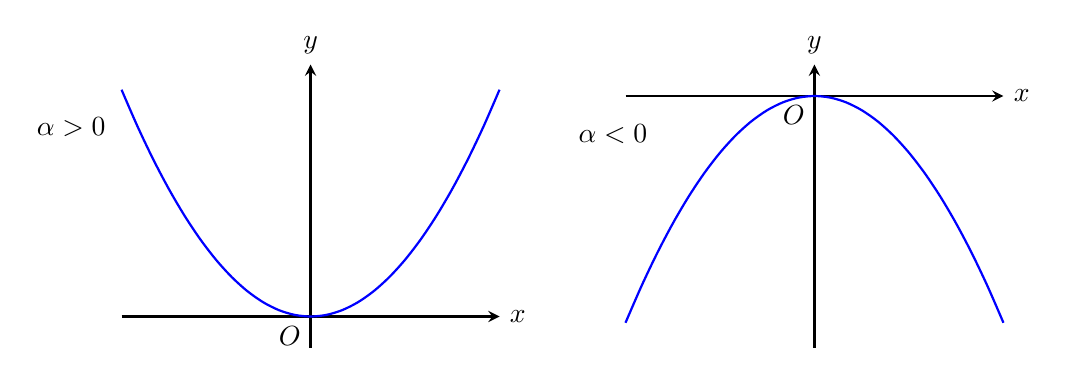
\begin{tikzpicture}[scale=0.8,>=stealth]

%%%%%%%%%%%%%%%%%%%%%%%%%%%%%%%%%%%%%%%%%%
  % Local scope
  \begin{scope}
    % Axes
    \draw[->, thick] (-3,0) -- (3,0) node[right] {$x$};
    \draw[->, thick] (0,-0.5) -- (0,4) node[above] {$y$};

    % Origin label
    \node[below left] at (0,0) {$O$};


    % Plot y = e^{x/5}
    \draw[domain=-3:3, smooth, variable=\x, blue, thick]
      plot ({\x},{0.4*(\x)^2});
    \node at (-3.8,3) {$\alpha > 0$};
  \end{scope}

%%%%%%%%%%%%%%%%%%%%%%%%%%%%%%%%%%%%%%%%%%

  \begin{scope}[xshift=8cm] % shift to the right
    % Axes
    \draw[->, thick] (-3,3.5) -- (3,3.5) node[right] {$x$};
    \draw[->, thick] (0,-0.5) -- (0,4) node[above] {$y$};

    % Origin
    \node[below left] at (0,3.5) {$O$};

    % Plot y = e^{x/5}
    \draw[domain=-3:3, smooth, variable=\x, blue, thick]
      plot ({\x},{-0.4*(\x)^2 + 3.5});
    \node at (-3.2,2.9) {$\alpha < 0$};
  \end{scope}

\end{tikzpicture}
\end{center}


\textbf{Η πολυωνυμική συνάρτηση $f(x) = {\alpha}x^3, \alpha \ne 0$}
\begin{center}
\begin{tikzpicture}[scale=0.8,>=stealth]

%%%%%%%%%%%%%%%%%%%%%%%%%%%%%%%%%%%%%%%%%%
  % Local scope
  \begin{scope}
    % Axes
    \draw[->, thick] (-3,0) -- (3,0) node[right] {$x$};
    \draw[->, thick] (0,-3) -- (0,3) node[above] {$y$};

    % Origin label
    \node[below left] at (0,0) {$O$};


    % Plot y = e^{x/5}
    \draw[domain=-2.8:2.8, smooth, variable=\x, blue, thick]
      plot ({\x},{0.15*(\x)^3});
    \node at (-3,3) {$\alpha > 0$};
  \end{scope}

%%%%%%%%%%%%%%%%%%%%%%%%%%%%%%%%%%%%%%%%%%

  \begin{scope}[xshift=9.1cm] % shift to the right
    % Axes
    \draw[->, thick] (-3,0) -- (3,0) node[right] {$x$};
    \draw[->, thick] (0,-3) -- (0,3) node[above] {$y$};

    % Origin
    \node[below left] at (0,0) {$O$};

    % Plot y = e^{x/5}
    \draw[domain=-2.8:2.8, smooth, variable=\x, blue, thick]
      plot ({\x},{-0.15*(\x)^3});

    \node at (-3.5,3) {$\alpha < 0$};

  \end{scope}

\end{tikzpicture}
\end{center}


\textbf{Η ρητή συνάρτηση $f(x) = \frac{\alpha}{x}, \alpha \ne 0$ και $D_{f} = \mathbb{R}^*$}
\begin{center}
\begin{tikzpicture}[scale=0.8,>=stealth]

%%%%%%%%%%%%%%%%%%%%%%%%%%%%%%%%%%%%%%%%%%
  % Local scope
  \begin{scope}
    % Axes
    \draw[->, thick] (-3,0) -- (3,0) node[right] {$x$};
    \draw[->, thick] (0,-3) -- (0,3) node[above] {$y$};

    % Origin label
    \node[below left] at (0,0) {$O$};


    % Plot y = e^{x/5}
    \draw[domain=0.17:2.8, smooth, variable=\x, blue, thick]
      plot ({\x},{0.5/(\x)});
    \draw[domain=-2.8:-0.17, smooth, variable=\x, blue, thick]
      plot ({\x},{0.5/(\x)});

    \node at (-2.6,3) {$\alpha > 0$};

  \end{scope}

%%%%%%%%%%%%%%%%%%%%%%%%%%%%%%%%%%%%%%%%%%

  \begin{scope}[xshift=9cm] % shift to the right
    % Axes
    \draw[->, thick] (-3,0) -- (3,0) node[right] {$x$};
    \draw[->, thick] (0,-3) -- (0,3) node[above] {$y$};

    % Origin
    \node[below left] at (0,0) {$O$};

    % Plot y = e^{x/5}
    \draw[domain=0.17:2.8, smooth, variable=\x, blue, thick]
      plot ({\x},{-0.5/(\x)});
    \draw[domain=-2.8:-0.17, smooth, variable=\x, blue, thick]
      plot ({\x},{-0.5/(\x)});

    \node at (-2.6,3) {$\alpha < 0$};
  \end{scope}

\end{tikzpicture}
\end{center}


\newpage

\textbf{Η συνάρτηση $f(x) = \sqrt{x}, \alpha \ne 0$ και $D_{f} = [0,+\infty)$}
\begin{center}
\begin{tikzpicture}[scale=0.8,>=stealth]

%%%%%%%%%%%%%%%%%%%%%%%%%%%%%%%%%%%%%%%%%%
  % Local scope
  \begin{scope}
    % Axes
    \draw[->, thick] (-0.5,0) -- (6,0) node[right] {$x$};
    \draw[->, thick] (0,-0.5) -- (0,5) node[above] {$y$};

    % Origin label
    \node[below left] at (0,0) {$O$};


    % Plot y = e^{x/5}
    \draw[domain=0:6, smooth, variable=\x, blue, thick]
      plot ({\x},{(\x)^(1/2)});

  \end{scope}
\end{tikzpicture}
\end{center}


\textbf{Η τριγωνομετρική συναρτήσεις: $f(x) = {\eta\mu}x + \beta$}
\begin{center}
\begin{tikzpicture}[scale=0.80, >=stealth]

  %%%%%%%%%%%%%%%%%%%%%%%%%%%%%%%%%%%%%%%%%%%%%%%%%
  \begin{scope}
    % Axes
    \draw[->, thick] (-0.5, 0) -- (2, 0) node[right] {$x$};
    \draw[->, thick] (0, -2) -- (0, 2) node[above] {$y$};

    % Plot function y = -sin(x) + 1.5
    \draw[domain=-2:1.5, smooth, variable=\x, blue, thick]
        plot ({\x},{sin(\x)});

    % Vertical dotted arrows to x-axis

    % Origin and labels
    \node[below left] at (0,0) {$O$};

    \node at (-2.2,2) {$\alpha > 0$};
  \end{scope}

  %%%%%%%%%%%%%%%%%%%%%%%%%%%%%%%%%%%%%%%%%%%%%%%%%
  \begin{scope}[xshift=7.2cm]
    % Axes
    \draw[->, thick] (-2, 0) -- (2, 0) node[right] {$x$};
    \draw[->, thick] (0, -2) -- (0, 2) node[above] {$y$};

    % Plot function
    \draw[domain=-1:1.7, smooth, variable=\x, blue, thick]
        plot ({\x},{cos(\x)});


    % Origin and labels
    \node[below left] at (0,0) {$O$};

    \node at (-2.2,2) {$\alpha < 0$};
  \end{scope}

  %%%%%%%%%%%%%%%%%%%%%%%%%%%%%%%%%%%%%%%%%%%%%%%%%
  \begin{scope}[xshift=14.3cm]
    % Axes
    \draw[->, thick] (-2, 0) -- (2, 0) node[right] {$x$};
    \draw[->, thick] (0, -2) -- (0, 2) node[above] {$y$};

    % Plot function
    \draw[domain=-2:2, smooth, variable=\x, blue, thick]
        plot ({\x},{0.5});


    \node[below left] at (0,0) {$O$};

    \node at (-2.2,2) {$\alpha = 0$};
  \end{scope}

\end{tikzpicture}
\end{center}


Τέλος, γνωρίζοντας την γραφική παράσταση μιας συνάρτησης (δηλαδή την $C_{f}$), μπορούμαι εύκολα να υπολογίσουμε την γραφική παράσταση μιας συνάρτησης σε αυτές τις περιπτώσεις, έστω υπάρχει $f(x)$:
\begin{enumerate}
 \item $-f(x)$
 \item $\vert f(x) \vert$
 \item $f(-x)$ (εφόσον $-x \in D_{f}$)
 \item $f(\vert x\vert)$ (εφόσον $\vert x\vert \in D_{f}$)
\end{enumerate}

Άρα έστω η παρακάτω γραφική παράσταση συνάρτησης, $C_{f}$:

\begin{center}
\begin{tikzpicture}[scale=0.8,>=stealth]

%%%%%%%%%%%%%%%%%%%%%%%%%%%%%%%%%%%%%%%%%%
  % Local scope
  \begin{scope}
    % Axes
    \draw[->, thick] (-2,0) -- (5,0) node[right] {$x$};
    \draw[->, thick] (0,-0.5) -- (0,5) node[above] {$y$};

    % Origin label
    \node[below right] at (0,0) {$O$};


    % Plot y = e^{x/5}
    \draw[domain=-0.74:3.8, smooth, variable=\x, blue, thick]
      plot ({\x},{-( ((-\x +1)/1.9)^7 + ((-\x +1)/1.9)^6 + ((-\x +1)/1.9)^2 + 2) + 2.7});

  \end{scope}
\end{tikzpicture}
\end{center}

Μπορούμαι να σχεδιάσουμε τις παρακάτω συναρτήσεις:

\begin{center}
\begin{tikzpicture}[scale=0.8,>=stealth]

%%%%%%%%%%%%%%%%%%%%%%%%%%%%%%%%%%%%%%%%%%
  % Local scope
  \begin{scope}
    % Axes
    \draw[->, thick] (-1.5,0) -- (4,0) node[right] {$x$};
    \draw[->, thick] (0,-3.6) -- (0,3.6) node[above] {$y$};

    % Origin label
    \node[below right] at (0,0) {$O$};


    \draw[domain=-1:3.7, dotted, variable=\x, blue, thick]
      plot ({\x},{-( ((-\x +1)/1.9)^7 + ((-\x +1)/1.9)^6 + ((-\x +1)/1.9)^2 + 2) + 2.7});
    \draw[domain=-1:3.7, smooth, variable=\x, blue, thick]
      plot ({\x},{( ((-\x +1)/1.9)^7 + ((-\x +1)/1.9)^6 + ((-\x +1)/1.9)^2 + 2) - 2.7});
    \node at (-1.9,-3.6) {(1)};

  \end{scope}

%%%%%%%%%%%%%%%%%%%%%%%%%%%%%%%%%%%%%%%%%%

  \begin{scope}[xshift=9cm] % shift to the right
    % Axes
    \draw[->, thick] (-1.5,0) -- (4,0) node[right] {$x$};
    \draw[->, thick] (0,-3.6) -- (0,3.6) node[above] {$y$};

    % Origin
    \node[below left] at (0,0) {$O$};


    \draw[domain=-1:3.7, dotted, variable=\x, blue, thick]
      plot ({\x},{-( ((-\x +1)/1.9)^7 + ((-\x +1)/1.9)^6 + ((-\x +1)/1.9)^2 + 2) + 2.7});
    \draw[domain=-1:3.7, samples=200, smooth, variable=\x, blue, thick]
      plot ({\x},{abs(-( ((-\x +1)/1.9)^7 + ((-\x +1)/1.9)^6 + ((-\x +1)/1.9)^2 + 2) + 2.7)});
    \node at (-1.9,-3.6) {(2)};
  \end{scope}

\end{tikzpicture}
\end{center}

\begin{center}
\begin{tikzpicture}[scale=0.8,>=stealth]

  \begin{scope} % shift to the right
    % Axes
    \draw[->, thick] (-4,0) -- (4,0) node[right] {$x$};
    \draw[->, thick] (0,-3.6) -- (0,3.6) node[above] {$y$};

    % Origin
    \node[below left] at (0,0) {$O$};

    \draw[domain=-1:3.7, dotted, variable=\x, blue, thick]
      plot ({\x},{-( ((-\x +1)/1.9)^7 + ((-\x +1)/1.9)^6 + ((-\x +1)/1.9)^2 + 2) + 2.7});
    \draw[domain=-1:3.7, smooth, variable=\x, blue, thick]
      plot ({-\x},{-( ((-\x +1)/1.9)^7 + ((-\x +1)/1.9)^6 + ((-\x +1)/1.9)^2 + 2) + 2.7});

    \node at (-3.5,-3.6) {(3)};
  \end{scope}

  \begin{scope}[xshift=9.1cm] % shift to the right
    % Axes
    \draw[->, thick] (-4,0) -- (4,0) node[right] {$x$};
    \draw[->, thick] (0,-3.6) -- (0,3.6) node[above] {$y$};

    % Origin
    \node[below right] at (0,0) {$O$};

    \draw[domain=-1:3.7, dotted, variable=\x, blue, thick]
      plot ({\x},{-( ((-\x +1)/1.9)^7 + ((-\x +1)/1.9)^6 + ((-\x +1)/1.9)^2 + 2) + 2.7});
    \draw[domain=-3.7:3.7, samples=200, smooth, variable=\x, blue, thick]
      plot ({\x},{-( ((-abs(\x) +1)/1.9)^7 + ((-abs(\x) +1)/1.9)^6 + ((-abs(\x) +1)/1.9)^2 + 2) + 2.7});

    \node at (-3.5,-3.6) {(4)};
  \end{scope}
\end{tikzpicture}
\end{center}



\textbf{ΠΡΟΣΟΧΗ!!!} Αν υποθέσουμε ότι το πεδίο ορισμού της συνάρτησης είναι αυτό που δόθηκε στο $C_f$, τότε: Οι δύο τελευταίες γραφικές παραστάσεις ((3),(4)) \textbf{\textit{δεν}} αναπαριστώνται στο πεδίο ορισμού που έχει δοθεί για το $C_f$.
